\section{Problem von Okamura und Seymour}

\texttt{KANTENDISJUNKTES WEGPACKUNGSPROBLEM}
\begin{itemize}
	\item \textbf{Gegeben}: Graph $G=(V,E)$ und Paare von Knoten $\{s_1,t_1\},\ldots,\{s_k,t_k\}, s_i,t_i\in V$
	\item \textbf{Gesucht}: Paarweise kantendisjunkter $s_i$-$t_i$-Wege $p_i$ in $G, 1 \leq i \leq k$
\end{itemize}
$s_i,t_i$ werden \textbf{Terminale} genannt, die Mengen $\{s_i,t_i\}$ heißen \textbf{Netze}.

Problem ist $\mathcal{NP}$-vollständig, auch falls $G$ planar ist. Wir werden das Problem deshalb später einschränken.\\

\textbf{Definition}: Sei $G=(V,E), X\subseteq V$. Dann heißt
$$\text{cap}(X)\coloneqq |\{uv\in E\mid u\in X, v\in V\setminus X\}|$$
die \textbf{Kapazität} von $X$. Zu $G$ sei $D=\{\{s_i,t_i\}\mid s_i,t_i\in V,1\leq i\leq k\}$ gegeben. Dann heißt
$$\text{dens}(X)\coloneqq|\{\{s_i,t_i\}\in D\mid |\{s_i,t_i\}\cap X|=1\}|$$
die \textbf{Dichte} von $X$. Weiterhin bezeichnet
$$\text{fcap}(X)\coloneqq \text{cap}(X)-\text{dens}(X)$$
die \textbf{freie Kapazität} von $X$. $X$ heißt \textbf{saturiert}, falls $\text{fcap}(X)=0$ und \textbf{übersaturiert}, falls $\text{fcap}(X)<0$.
\begin{center}
	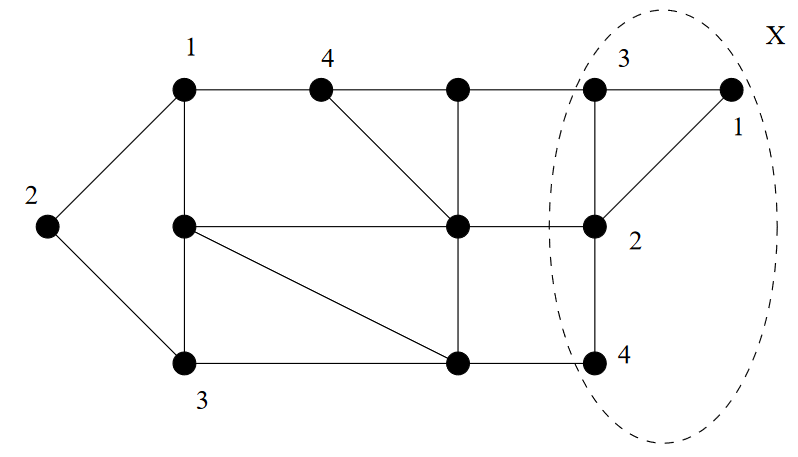
\includegraphics[width=0.4\textwidth]{images/s1.png}
\end{center}
\pagebreak
\textbf{Definition}:
\begin{itemize}
	\item \textbf{Kapazitätsbedingung}: $\text{fcap}(X)\geq 0$ für alle $X\subseteq V$. Jedes lösbare \texttt{KANTENDISJUNKTE WEGPACKUNGSPROBLEM} erfüllt die Bedingung, aber nicht jedes Problem, das die Bedingung erfüllt, ist lösbar.
	\begin{center}
		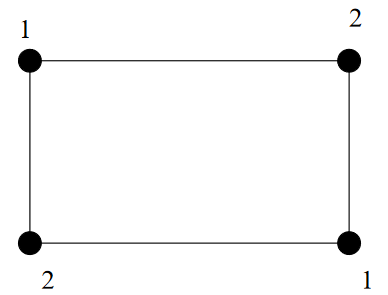
\includegraphics[width=0.2\textwidth]{images/s2.png}
	\end{center}
	$\text{cap}(X)\geq 2$ für alle $X\neq \emptyset$ und $\text{dens}(X)\leq 2$, aber nicht lösbar
	\item \textbf{Geradheitsbedingung}: $\text{fcap}(X)$ ist gerade für alle $x\subseteq V$
\end{itemize}
\bigskip
\textbf{Lemma}: Sei $G=(V,E)$ und $D=\{\{s_i,t_i\}\mid s_i,t_i\in V,1\leq i\leq k\}$. Es gilt $\text{fcap}(X)$ gerade für alle $X\subseteq V$ $\iff \text{fcap}(v)\coloneqq\text{fcap}(\{v\})$ gerade für alle $v\in V$

\textit{Beweis}:
\begin{itemize}
	\item \enquote{$\Rightarrow$}: Trivial.
	\item \enquote{$\Leftarrow$}: Sei $\text{fcap}(v)$ gerade für alle $v\in V$. Für $X\subseteq V$ ist
	\begin{itemize}
		\item $\text{cap}(X)=\sum\limits_{v\in X} \text{cap}(v)-2\cdot |\{uv\in E\mid u,v\in X\}|$
		\item $\text{dens}(X)=\sum\limits_{v\in X}\text{dens}(v)-2\cdot |\{\{s_i,t_i\}\in D\mid s_i,t_i\in X\}|$
	\end{itemize}
	Dann ist:
	$$
	\begin{aligned}
		\operatorname{fcap}(X)= & \sum_{v \in X} \operatorname{cap}(v)-\sum_{v \in X} \operatorname{dens}(v)-2 \cdot|\{uv \in E: u, v \in X\}| \\
		& +2\cdot\left|\left\{\left\{s_{i}, t_{i}\right\} \in D: s_{i}, t_{i} \in X\right\}\right| \\
		= & \sum_{v \in X} \operatorname{fcap}(v)-2 \cdot(|\{uv \in E: u, v \in X\}| \\
		& \left.+2\cdot\left|\left\{\left\{s_{i}, t_{i}\right\} \in D: s_{i}, t_{i} \in X\right\}\right|\right)
	\end{aligned}
	$$
	Also ist $\text{fcap}(X)$ gerade, falls alle $\text{fcap}(v)$ gerade sind.
\end{itemize}